\documentclass[12pt]{article}
\usepackage{graphicx} %required for inserting images
\graphicspath{{./images/}}
\usepackage{array}
\usepackage{lipsum}
\usepackage{amsmath}
\title{GEOTECHNICAL DESIGN OF DRIVEN PILES UNDER AXIAL LOADS}
\author{Sakib Bin Rafi Tonmoy,Jakaria Pervez}
\date{05/04/2023}
\begin{document}
\maketitle

%%Begining of Introduction
\section{Settlement of Floating Piles}
 If concrete columns are not end bearing, the settlement may become an issue. The settlement of concrete column-reinforced soft foundations can be estimated using the method for piled rafts or pile groups.Horikoshi and Randolph (1999) and Poulos (2001) proposed simplified design methods to calculate the settlement of piled rafts, which are based on pile–raft interaction. \\
 
 
 %%adding figure for equivalent pier
\begin{figure}[h]
\centering
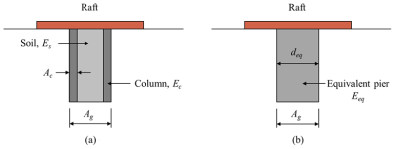
\includegraphics{Equivalent_Pier}
\caption{Equivalent Pier}
\label{fig:eqv_pier}
\end{figure}

%%end of figure


Randolph (1999) used the equivalent pier concept for the piled raft method as shown in \ref{fig:eqv_pier}


%%End of Introduction of Introduction



\section{API Procedure}
%\lipsum[2]
%writing necessary equation





\begin{center}
\begin{table}
\begin{tabular}{|m{10cm}|m{2cm}|m{4cm}|}
\hline
soil & \delta,degrees & Limiting f,kips/fit^2(kPa) \\
\hline
Very loose & 15 & 1.0 (47.8)\\
\hline
Loose & 20 & 1.4 (67.0)\\
\hline
Medium & 25 & 1.7 (83.1)\\
\hline
Dense & 30 & 2.0 (95.5)\\
\hline
\end{tabular}
\caption{\label{f_non_cohesive}uideline for Side Friction in Siliceous Soil}
\end{table}

\end{center}
\end{document}